% !TeX program = xelatex
% Journal-style author manuscript, not an official publisher class.
% Compile main.tex from this directory with XeLaTeX (twice) or Tectonic.
\documentclass[UTF8,a4paper,twocolumn,fontset=none,zihao=5]{ctexart}
\usepackage[top=20mm,bottom=20mm,left=18mm,right=18mm,columnsep=7mm]{geometry}
\usepackage{amsmath,amssymb,booktabs,graphicx,tabularx,array}
\usepackage{caption,enumitem,needspace,balance}
\usepackage{cite}
\newcommand{\upcite}[1]{\textsuperscript{\cite{#1}}}
\usepackage{xurl}
\usepackage[hidelinks,bookmarksnumbered]{hyperref}
\IfFontExistsTF{SimSun}{\setCJKmainfont{SimSun}[AutoFakeBold=2]}{\setCJKmainfont{FandolSong-Regular}[BoldFont=FandolSong-Bold]}
\IfFontExistsTF{SimHei}{\setCJKsansfont{SimHei}[AutoFakeBold=2]}{\setCJKsansfont{FandolHei-Regular}[BoldFont=FandolHei-Bold]}
\IfFontExistsTF{SimSun}{\setCJKmonofont{SimSun}}{\setCJKmonofont{FandolSong-Regular}}
\setmainfont{texgyretermes-regular.otf}[BoldFont=texgyretermes-bold.otf,ItalicFont=texgyretermes-italic.otf,BoldItalicFont=texgyretermes-bolditalic.otf]
\setsansfont{texgyreheros-regular.otf}[BoldFont=texgyreheros-bold.otf]
\ctexset{section={format=\large\sffamily\bfseries,beforeskip=9pt,afterskip=5pt},
 subsection={format=\normalsize\sffamily\bfseries,beforeskip=7pt,afterskip=3pt}}
\setlength{\parindent}{2em}
\setlength{\parskip}{0pt}
\linespread{1.04}
\setlength{\abovedisplayskip}{5pt plus 1pt minus 1pt}
\setlength{\belowdisplayskip}{5pt plus 1pt minus 1pt}
\setlength{\textfloatsep}{10pt plus 2pt minus 2pt}
\setlength{\dbltextfloatsep}{10pt plus 2pt minus 2pt}
\setlength{\floatsep}{8pt plus 2pt minus 2pt}
\renewcommand{\topfraction}{0.93}
\renewcommand{\dbltopfraction}{0.93}
\renewcommand{\textfraction}{0.06}
\renewcommand{\floatpagefraction}{0.80}
\renewcommand{\dblfloatpagefraction}{0.80}
\setcounter{topnumber}{3}
\setcounter{dbltopnumber}{3}
\makeatletter
\setlength{\@fptop}{0pt}
\setlength{\@fpsep}{10pt}
\setlength{\@fpbot}{0pt plus 1fil}
\makeatother
\captionsetup{font=small,labelsep=quad,skip=4pt}
\setlist[enumerate]{leftmargin=1.8em,nosep,label=\arabic*.}
\newcolumntype{Y}{>{\centering\arraybackslash}X}
\newcommand{\algtitle}[1]{\par\Needspace{6\baselineskip}\smallskip\noindent\textbf{#1}\par\smallskip}
\emergencystretch=1em
\raggedbottom
\pagestyle{plain}
\setcounter{section}{-1}
\hypersetup{pdftitle={资源匹配下超图支付网络的服务可靠性},pdfauthor={作者待填}}


\begin{document}

\onecolumn

\renewcommand{\thefigure}{S\arabic{figure}}

\section*{S5：四臂补充图及读图说明}

本补充复用已核验的四臂统计，不产生新的模拟或重抽样。每相位、每规模60父图，3模型各20，7条轨迹先在父图内平均；所有条件均保留。U为节点预算均匀初态，O为原优化初态。两相位标签仅指数据来源，本补充为事后分析。

统计使用Python 3.12.14。每相位、每规模20\,000次模型分层整父图配对bootstrap，四臂及两个终点共享索引；每模型抽20父图有放回，以模型均值等权汇总。种子2026100705及SHA-256派生副本/模型种子，点估计和区间保留精确有理数；区间为逆经验分布第500和19\,500顺序统计量，点态95\%、未校正，无p值。全部160\,000次副本已经单独算术核验，但该核验不是独立盲科学审查。

\begin{figure}[ht]\centering

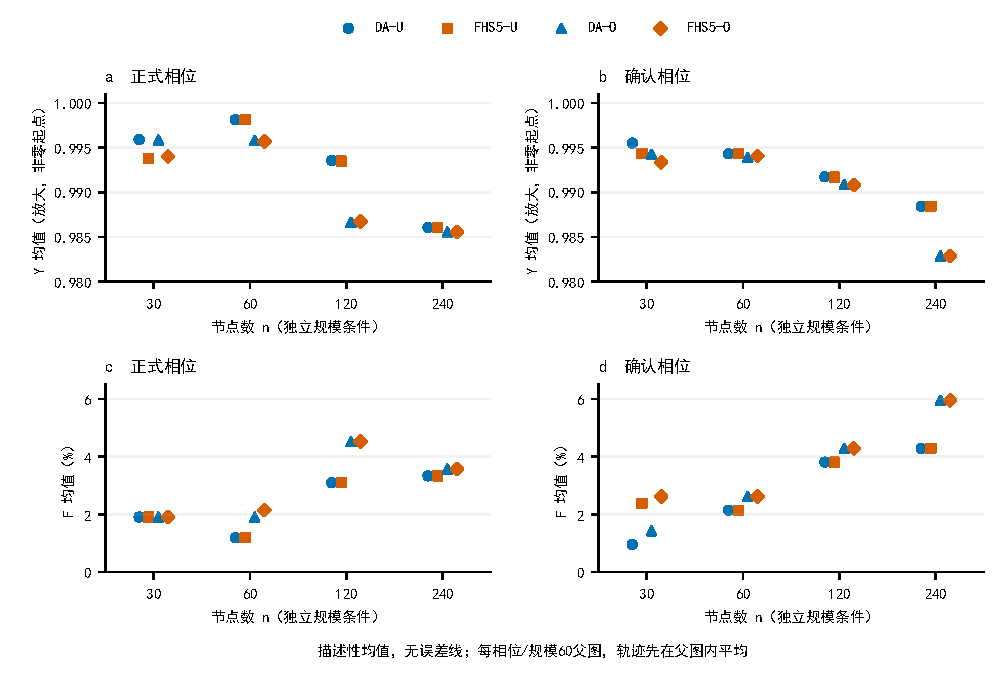
\includegraphics[width=170mm]{figures/s5-arm-means.pdf}

\caption{四臂绝对均值。a、b为正式与确认相位Y均值，c、d为F均值（百分数）。Y轴放大且非零起点，F轴从零开始；不画误差线。标记只表示各独立规模条件，不连接为时间轨迹。每父图7条轨迹先汇总，3模型等权。图的作用是给出差值所在的绝对水平，不证明臂间等效。}

\end{figure}

\clearpage

\begin{figure}[ht]\centering

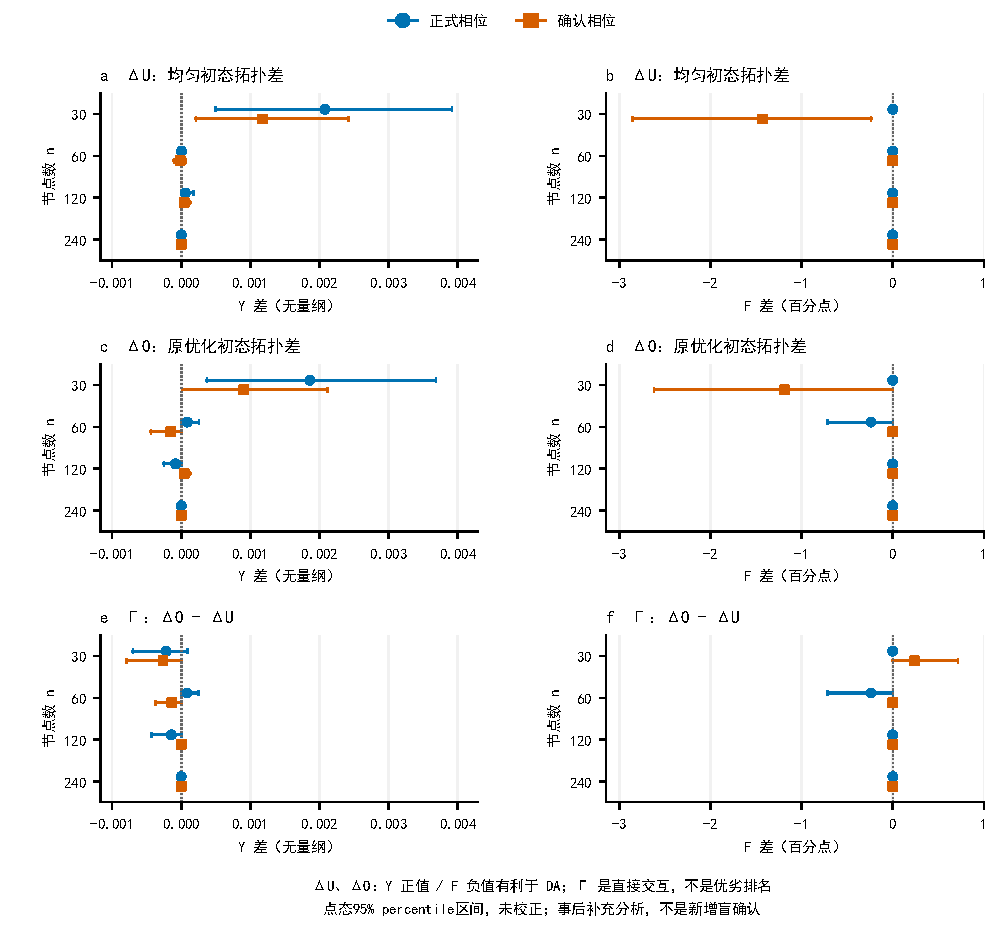
\includegraphics[width=170mm]{figures/s5-topology-interaction.pdf}

\caption{拓扑对比与直接交互。a、b为均匀初态的DA减FHS5，c、d为原优化初态对应差，e、f为两种拓扑差之差。左列为Y差（无量纲），右列为F差（百分点）；圆点为正式、方块为确认。横线是共享索引、模型分层、整父图20\,000次重抽样所得点态95\% percentile区间，未校正。共48项完整合并范围对比；交互不是由显著性有无推断。零宽经验区间不证明总体等效。}

\end{figure}

\clearpage

\begin{figure}[ht]\centering

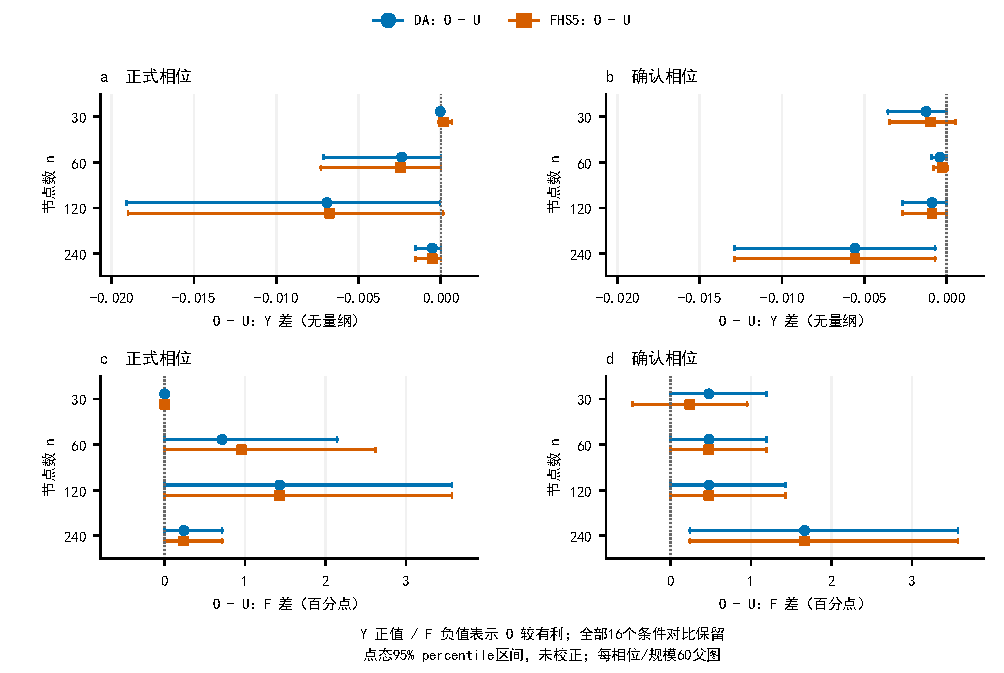
\includegraphics[width=170mm]{figures/s5-initialization.pdf}

\caption{各拓扑内部的初态对比。a、b为正式、确认相位Y差，c、d为对应F差（百分点）。圆点为DA、方块为FHS5的O减U，横线为点态、未校正95\%区间。共32项完整合并范围对比；Y正值和F负值表示O较有利。16个时间条件中15负1正只是描述性方向计数，不是16个独立重复或多重校正结论。}

\end{figure}

\section*{源数据和边界}

完整源数据保留240项对比和192项四臂均值，包括160项无区间的同分布、偏移描述对比及128项范围均值。主分析的40项家族复现判据与本补充80项点态区间不同，不得合并解释。Y为首次无路径请求索引截断至H后除以H；末次请求发生事件与窗口内无事件的Y可能相同，但F不同。风险百分点差不是相对风险百分比。固定的是节点初始预算而非每条超边资金，因此图形不识别纯拓扑因果效应。

\end{document}